\chapter{Fonctions usuelles}
\section{Fonctions polynomiales}
\begin{graybox}
	\begin{definition}[Fonction polynomiale]
		\par Soient $n \in \N$ et $a_0, a_1, \ldots, a_n$ des réels.
		\par La fonction :
		\begin{align*}
			f : 
			\begin{cases}
				\R &\to \R \\
				x &\mapsto \sum_{k = 0}^{n}a_kx^k = a_0 x^0 + a_1 x^1 + \cdots + a_n x^n
			\end{cases}
		\end{align*}
		\par est une fonction polynomiale de degré $n$.
		\par Cette fonction est dérivable.
		\begin{align*}
			f'(x) = \sum_{k=1}^{n}ka_kx^{k-1} = a_1 + 2a_2x + \cdots + na_nx^{n-1}
		\end{align*}
	\end{definition}
\end{graybox}

\begin{remarque}
	La somme, le produit et la composition de fonctions polynomiales sont des fonctions polynomiales.
\end{remarque}

\begin{graybox}
	\begin{proposition}[]
		\par Soit $f:\R \to \R$ une fonction polynomiale de degré $n$
		\begin{itemize}
			\item $n = 0$, on obtient les fonctions constantes, pour $a_0 \in \R$
			\begin{align*}
				f:
				\begin{cases}
					\R &\to \R \\
					x &\mapsto a_0
				\end{cases}
			\end{align*}
			\item $n = 1$, on obtient les fonctions affines, pour $(a, b) \in \R^2$
			\begin{align*}
				f:
				\begin{cases}
					\R &\to \R \\
					x &\mapsto ax + b
				\end{cases}
			\end{align*}
			\item $n = 2$, on obtient les fonctions trinômes, pour $(a, b, c) \in \R^3$
			\begin{align*}
				f:
				\begin{cases}
					\R &\to \R \\
					x &\mapsto ax^2 + bx + c
				\end{cases}
			\end{align*}
		\end{itemize}
	\end{proposition}
\end{graybox} 


\begin{remarque}~
	\begin{itemize}
		\item Les fonctions constantes sont les seules fonctions à la fois croissantes et décroissantes.
		\item Une fonction dérivable de dérivée nulle est constante.
		\item Une fonction dérivable de dérivée constante est affine.
	\end{itemize}
\end{remarque}


\section{Fonction partie entière $E$}
\begin{graybox}
	\begin{definition}[Fonction partie entière $E$]
		\begin{align*}
			\forall x \in \R,\exists!E(x) \in \Z, E(x) \leq x < E(x+1)
		\end{align*}
		$E(x)$ est la partie entière de $x$
		\begin{align*}
			E :
			\begin{cases}
				\R &\to \Z \\
				x &\mapsto E(X)
			\end{cases}
		\end{align*}
	\end{definition}
\end{graybox}


\begin{figure}[h!]
	\centering
	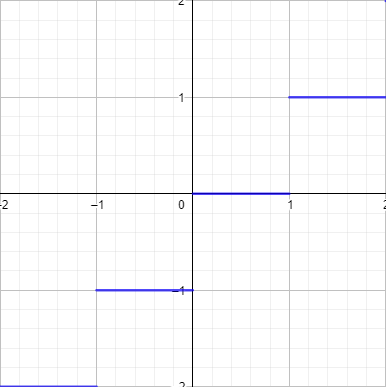
\includegraphics[scale=0.5]{images/partie_entiere.png}
	\caption{Partie entière}
\end{figure}

\begin{remarque}~
	\begin{itemize}
		\item E est croissante.
		\item E est non-continue en tout point de $\Z$.
		\item $x \mapsto x - E(x)$ est 1-périodique.
		\item $E^{-1}(\{0\}) = [0, 1[$.
	\end{itemize}
\end{remarque}


\section{Fonctions trigonométriques}
\begin{table}[h!]
	\centering
	\begin{tabular}{c c c c}
		\textbf{Fonction}
		& $f :\begin{cases}
			\R &\to \R \\    
			x &\mapsto \cos{x}
		\end{cases}$
		& $f :\begin{cases}
			\R &\to \R \\    
			x &\mapsto \sin{x}
		\end{cases}$
		& $f :\begin{cases}
			\R &\to \R \\    
			x &\mapsto \tan{x} = \frac{\sin{x}}{\cos{x}}
		\end{cases}$
		\\
		\hline
		\textbf{Parité} & Paire & Impaire & Impaire \\
		\textbf{Périodicité} & $2\pi\textnormal{-périodique}$ & $2\pi\textnormal{-périodique}$ & $\pi\textnormal{-périodique}$ \\
		\textbf{Dérivée} & $x \mapsto -\sin{x}$ & $x \mapsto \cos{x}$ & $x \mapsto \frac{1}{\cos^2{x}} = 1 + \tan^2{x}$ \\
		\textbf{Primitive} & $x \mapsto \sin{x}$ & $x\mapsto -\cos{x}$ & $x \mapsto - \ln{|\cos{x}|}$ \\
		\hline
	\end{tabular}
	\caption{Fonctions trigonométriques}
\end{table}


\begin{remarque}
	\par On peut éventuellement considérer l'ensemble d'arrivée de $\sin$ et $\cos$ comme étant $[-1,1]$
\end{remarque}


\begin{figure}[h!]
	\centering
	%\includegraphics{images/cos.png}
	\begin{subfigure}{0.3\textwidth}
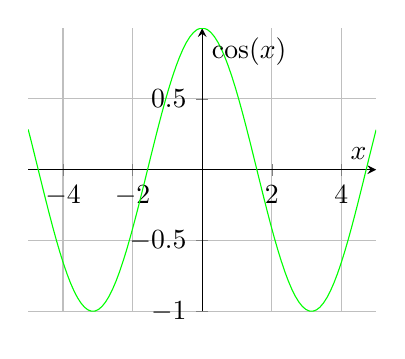
\begin{tikzpicture}
            \begin{axis}[domain=-5:5, axis lines=middle, grid=both, xlabel=$x$, ylabel=$\cos(x)$, width=6cm]
                \addplot[color=green, samples=100] {cos(deg(x))};
            \end{axis}
    \end{tikzpicture}
		
		\caption{Fonction $\cos{x}$}
	\end{subfigure}
	\begin{subfigure}{0.3\textwidth}
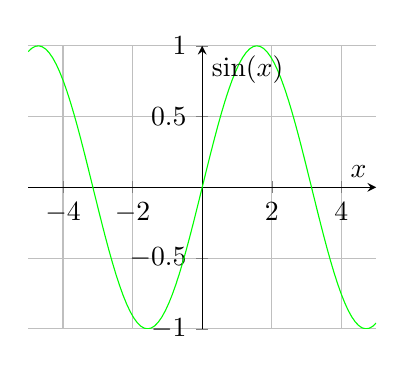
\begin{tikzpicture}
            \begin{axis}[domain=-5:5, axis lines=middle, grid=both, xlabel=$x$, ylabel=$\sin(x)$, width=6cm]
                \addplot[color=green, samples=100] {sin(deg(x))};
            \end{axis}
    \end{tikzpicture}
		\caption{Fonction $\sin{x}$}
	\end{subfigure}
	\begin{subfigure}{0.3\textwidth}
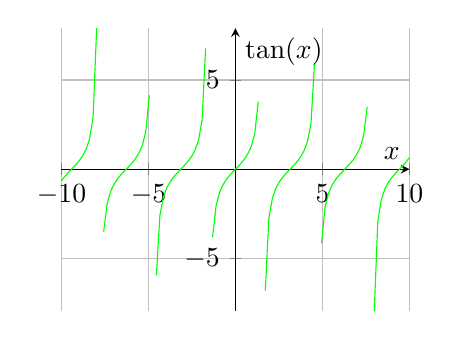
\begin{tikzpicture}
            \begin{axis}[domain=-10:10, restrict y to domain=-10:10, axis lines=middle, grid=both, xlabel=$x$, ylabel=$\tan(x)$, width=6cm]
                \addplot[color=green, samples=100] {tan(deg(x))};
            \end{axis}
    \end{tikzpicture}
		\caption{Fonction $\tan{x}$}
	\end{subfigure}
\end{figure}

\begin{graybox}
	\begin{proposition}[Formules trigonométriques]
		$\forall x \in \R$ (il est possible de retrouver ces formules géométriquement)
		\begin{itemize}
			\item $\cos{x} = \cos{(-x)}$
			\item $\sin{(-x)} = -\sin{x}$
			\item $\cos{(\pi - x)} = -\cos{x}$
			\item $\sin{(\pi - x)} = \sin{x}$
			\item $\cos{(\pi + x)} = -\cos{x}$
			\item $\sin{(\pi + x)} = -\sin{x}$
			\item $\cos{(\frac{\pi}{2} - x)} = \sin{x}$
			\item $\sin{(\frac{\pi}{2} - x)} = \cos{x}$
			\item $\cos{(\frac{\pi}{2} + x)} = -\sin{x}$
			\item $\sin{(\frac{\pi}{2} + x)} = -\cos{x}$
		\end{itemize}
	\end{proposition}
\end{graybox}

% La base du code définissant le cercle trigonométrique provient de : https://texemple.net/tikz/exemples/unit-circle/
\begin{figure}[h!]
	\centering
	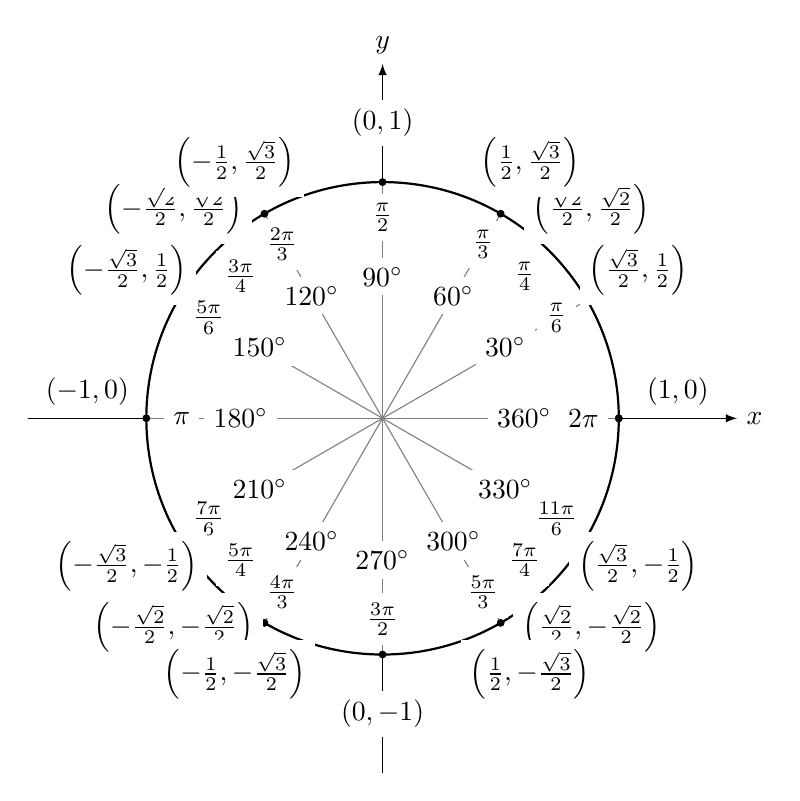
\begin{tikzpicture}[scale=3,cap=round,>=latex]
		% draw the coordinates
		\draw[->] (-1.5cm,0cm) -- (1.5cm,0cm) node[right,fill=white] {$x$};
		\draw[->] (0cm,-1.5cm) -- (0cm,1.5cm) node[above,fill=white] {$y$};
		
		% draw the unit circle
		\draw[thick] (0cm,0cm) circle(1cm);
		
		\foreach \x in {0,30,...,360} {
			% lines from center to point
			\draw[gray] (0cm,0cm) -- (\x:1cm);
			% dots at each point
			\filldraw[black] (\x:1cm) circle(0.4pt);
			% draw each angle in degrees
			\draw (\x:0.6cm) node[fill=white] {$\x^\circ$};
		}
		
		% draw each angle in radians
		\foreach \x/\xtext in {
			30/\frac{\pi}{6},
			45/\frac{\pi}{4},
			60/\frac{\pi}{3},
			90/\frac{\pi}{2},
			120/\frac{2\pi}{3},
			135/\frac{3\pi}{4},
			150/\frac{5\pi}{6},
			180/\pi,
			210/\frac{7\pi}{6},
			225/\frac{5\pi}{4},
			240/\frac{4\pi}{3},
			270/\frac{3\pi}{2},
			300/\frac{5\pi}{3},
			315/\frac{7\pi}{4},
			330/\frac{11\pi}{6},
			360/2\pi}
		\draw (\x:0.85cm) node[fill=white] {$\xtext$};
		
		\foreach \x/\xtext/\y in {
			% the coordinates for the first quadrant
			30/\frac{\sqrt{3}}{2}/\frac{1}{2},
			45/\frac{\sqrt{2}}{2}/\frac{\sqrt{2}}{2},
			60/\frac{1}{2}/\frac{\sqrt{3}}{2},
			% the coordinates for the second quadrant
			150/-\frac{\sqrt{3}}{2}/\frac{1}{2},
			135/-\frac{\sqrt{2}}{2}/\frac{\sqrt{2}}{2},
			120/-\frac{1}{2}/\frac{\sqrt{3}}{2},
			% the coordinates for the third quadrant
			210/-\frac{\sqrt{3}}{2}/-\frac{1}{2},
			225/-\frac{\sqrt{2}}{2}/-\frac{\sqrt{2}}{2},
			240/-\frac{1}{2}/-\frac{\sqrt{3}}{2},
			% the coordinates for the fourth quadrant
			330/\frac{\sqrt{3}}{2}/-\frac{1}{2},
			315/\frac{\sqrt{2}}{2}/-\frac{\sqrt{2}}{2},
			300/\frac{1}{2}/-\frac{\sqrt{3}}{2}}
		\draw (\x:1.25cm) node[fill=white] {$\left(\xtext,\y\right)$};
		
		% draw the horizontal and vertical coordinates
		% the placement is better this way
		\draw (-1.25cm,0cm) node[above=1pt] {$(-1,0)$}
		(1.25cm,0cm)  node[above=1pt] {$(1,0)$}
		(0cm,-1.25cm) node[fill=white] {$(0,-1)$}
		(0cm,1.25cm)  node[fill=white] {$(0,1)$};
	\end{tikzpicture}
	\caption{Cercle trigonométrique : \cite{cercle_trigo}}
\end{figure}
% Fin du code emprunté 



\begin{table}[h!]
	\centering
	\begin{tabular}{c c c c c c}
		$x$ & $0$ & $\frac{\pi}{6}$ & $\frac{\pi}{4}$ & $\frac{\pi}{3}$ & $\frac{\pi}{2}$ \\
		\hline
		$\cos{x}$ & 1 & $\frac{\sqrt{3}}{2}$ & $\frac{\sqrt{2}}{2}$ & $\frac{1}{2}$ & 0 \\
		$\sin{x}$ & 0 & $\frac{1}{2}$ & $\frac{\sqrt{2}}{2}$ & $\frac{\sqrt{3}}{2}$ & 1 \\
		$\sin^2{x}$ & 0 & $\frac{1}{4}$ & $\frac{2}{4}$ & $\frac{3}{4}$ & 1 \\ 
		\hline
	\end{tabular}
	\caption{Valeurs remarquables}
\end{table}

\begin{graybox}
	\begin{proposition}[Formules d'addition]
		$\forall (a, b) \in \R^2$
		\begin{align*}
			&\sin{(a+b)} = \sin{(a)}\cos{(b)} + \sin{(b)}\cos{(a)} \\
			&\cos{(a+b)} = \cos{(a)}\cos{(b)} - \sin{(a)}\sin{(b)}
		\end{align*}
	\end{proposition}
\end{graybox}

\begin{remarque}{En particulier pour $a=b$}~
	\begin{itemize}
		\item $\sin{(2a)} = 2 \sin{a}\cos{a}$
		\item $\cos{(2a)} = \cos^2{a}-\sin^2{a}$
		\item $\cos{(2a)} = 1 - 2\sin^2{a}$
		\item $\cos{(2a)} = 2\cos^2{a} - 1$
	\end{itemize}
	On en déduit :
	\begin{align*}
		\cos^2{a} &= \frac{1 + \cos{(2a)}}{2} & \sin^2{a} &= \frac{1 - \cos{(2a)}}{2}
	\end{align*}
\end{remarque}

\begin{remarque}[Mnémotechnique]~
	\\
	"cosinus est une fonction \textbf{raciste} et \textbf{menteuse}" 
	\begin{itemize}
		\item \textbf{Menteuse} : Elle change le signe
		\item \textbf{Raciste} : Elle ne mélange pas sinus et cosinus
	\end{itemize}
\end{remarque}

\section{Fonctions trigonométriques réciproques}
\begin{remarque}
	On cherche à changer l'ensemble de départ et d'arrivée pour rendre les fonctions trigonométriques bijectives.
\end{remarque}

\begin{graybox}
	\begin{proposition}[]
		Les fonctions :
		\begin{itemize}
			\item $\sin : [-\frac{\pi}{2}, \frac{\pi}{2}] \to [-1, 1]$
			\item $\cos : [0, \pi] \to [-1,1]$
			\item $\tan : ]-\frac{\pi}{2}, \frac{\pi}{2}[ \to \R$
		\end{itemize}
		sont bijectives.
	\end{proposition}
\end{graybox}

\begin{graybox}
	\begin{proposition}[]
		On peut définir leurs bijections réciproques :
		\begin{itemize}
			\item $\arcsin : [-1,1] \to [-\frac{\pi}{2},\frac{\pi}{2}]$
			\item $\arccos : [-1,1] \to [0, \pi]$
			\item $\arctan : \R \to ]-\frac{\pi}{2},\frac{\pi}{2}[$
		\end{itemize}
	\end{proposition}
\end{graybox}

\begin{graybox}
	\begin{proposition}[]
		On a alors : 
		\begin{itemize}
			\item $\forall x \in [-\frac{\pi}{2}, \frac{\pi}{2}], \arcsin{(\sin{x})} = x $
			\item $\forall x \in [0, \pi], \arccos{(\cos{x})} = x$
			\item $\forall x \in ]-\frac{\pi}{2}, \frac{\pi}{2}[, \arctan{(\tan{x})} = x$
		\end{itemize}
	\end{proposition}
\end{graybox}

\begin{graybox}
	\begin{proposition}[]
		\begin{align*}
			&\forall y \in [-1,1] 
			\begin{cases}
				\sin{(\arcsin{y})} = y \\
				\cos{(\arccos{y})} = y
			\end{cases}
			\\
			&\forall y \in \R \tan{(\arctan{y})} = y
		\end{align*}
	\end{proposition}
\end{graybox}

\begin{remarque}
	Les graphes des fonctions réciproques s'obtiennent par réflexion par rapport à la droite $y =x $
\end{remarque}

\begin{graybox}
	\begin{proposition}{Valeurs remarquables}
		\begin{itemize}
			\item $\arcsin{(1)} = \frac{\pi}{2}$
			\item $\arcsin{(0)} = 0$
			\item $\arcsin{(-1)} = -\frac{\pi}{2}$
			\item $\arccos{(1)} = 0$
			\item $\arccos{(0)} = \frac{\pi}{2}$
			\item $\arccos{(-1)} = \pi$
		\end{itemize}
	\end{proposition}
\end{graybox}

\begin{figure}[h!]
	\centering
	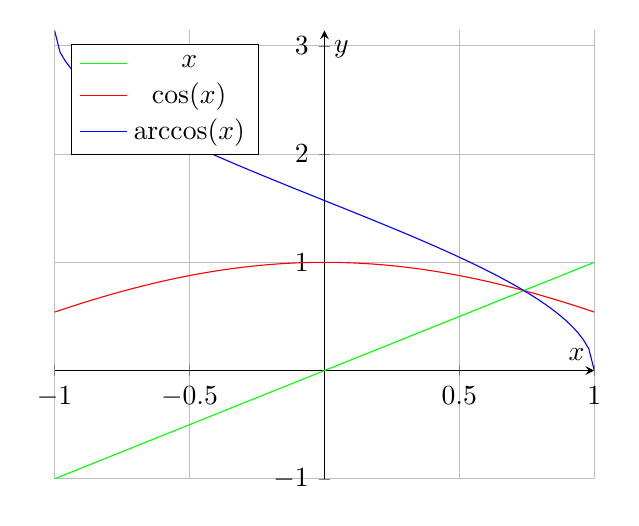
\begin{tikzpicture}
		\begin{axis}[domain=-1:1, axis lines=middle, grid=both, xlabel=$x$, ylabel=$y$, samples=100, legend pos=north west]
			\addplot[color=green]{x};
			\addlegendentry{$x$}
			\addplot[color=red]  {cos(deg(x))};
			\addlegendentry{$\cos(x)$}
			\addplot[color=blue]  {rad(acos(x))};
			\addlegendentry{$\arccos(x)$}
		\end{axis}
	\end{tikzpicture}
\end{figure}

\begin{figure}[h!]
	\centering
	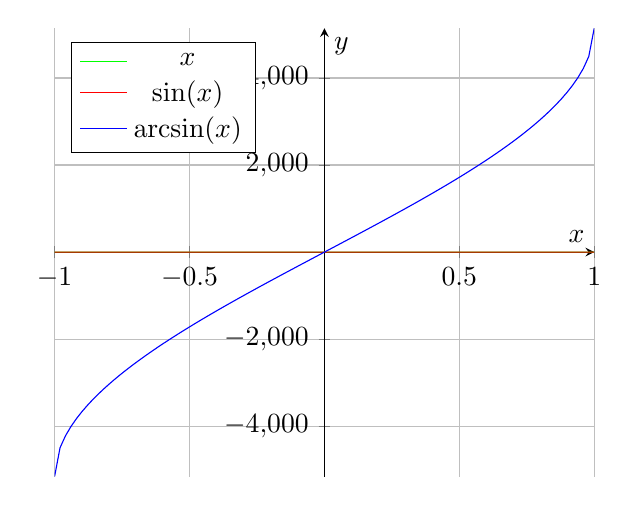
\begin{tikzpicture}
		\begin{axis}[domain=-1:1, axis lines=middle, grid=both, xlabel=$x$, ylabel=$y$, samples=100, legend pos=north west]
			\addplot[color=green]{x};
			\addlegendentry{$x$};
			\addplot[color=red]  {sin(deg(x))};
			\addlegendentry{$\sin(x)$};
			\addplot[color=blue]  {deg(asin(x))};
			\addlegendentry{$\arcsin(x)$};
		\end{axis}
	\end{tikzpicture}
\end{figure}

\begin{figure}[h!]
	\centering
	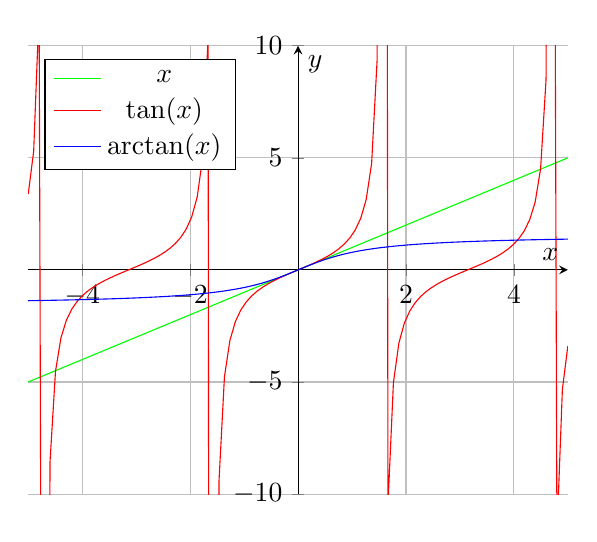
\begin{tikzpicture}
		\begin{axis}[xmin=-5, xmax=5, ymin=-10, ymax=10, axis lines=middle, grid=both, xlabel=$x$, ylabel=$y$, samples=100, legend pos=north west]
			\addplot[color=green]{x};
			\addlegendentry{$x$};
			\addplot[color=red]  {tan(deg(x))};
			\addlegendentry{$\tan(x)$};
			\addplot[color=blue]  {rad(atan(x))};
			\addlegendentry{$\arctan(x)$};
		\end{axis}
	\end{tikzpicture}
\end{figure}


\begin{table}[h!]
	\centering
	\begin{tabular}{c c c c}
		\textbf{Fonction}& $\arcsin$ & $\arccos$ & $\arctan$ \\
		\hline
		\textbf{Monotonie} & Croissante & Décroissante & Croissante \\
		\textbf{Parité} & Impaire & $\emptyset$ & Impaire \\
		\hline
	\end{tabular}
	\caption{Monotonie et parité des fonctions trigonométriques réciproques}
\end{table}    

\begin{graybox}
	\begin{proposition}[Limite de $\arctan$]
		\begin{align*}
			\lim_{x \to +\infty}{\arctan{x}} &= \frac{\pi}{2} & \lim_{x \to -\infty}{\arctan{x}} &= -\frac{\pi}{2}
		\end{align*}
	\end{proposition}
\end{graybox}

\begin{graybox}
	\begin{proposition}[Dérivées]
		\begin{align*}
			1.\ \forall x \in ]-1, 1[ \ \arcsin'{x} = \frac{1}{\sqrt{1 - x^2}} 
		\end{align*}
		\begin{align*}
			2. \ \forall x \in [-1, 1] \ \arccos'{x} = - \frac{1}{\sqrt{1 - x^2}} 
		\end{align*}
		\begin{align*}
			3. \ \forall x \in \R \ \arctan'{x} = \frac{1}{1 + x^2}
		\end{align*}
	\end{proposition}
\end{graybox}

\begin{proof}
	1.
	\begin{align*}
		&\forall y \in [-1, 1] \textnormal{ on a : } \sin(\arcsin(y)) = y \\
		&\textnormal{Donc on a : } \cos^2(\arcsin(y)) + \underbrace{\sin^2(\arcsin(y))}_{=y^2} = 1 \\
		&\cos^2(\arcsin(y)) = 1 - y^2 \\
		&\arcsin(y) \in [-\frac{\pi}{2}, \frac{\pi}{2}] \textnormal{ donc } \cos(\arcsin(y)) > 0 \\
		&\textnormal{on en déduit } \cos(\arcsin(y)) = \sqrt{1 - y^2} \\
		&\textnormal{En dérivant on obtient : } \arcsin'(y) \times \underbrace{(-\sin(\arcsin(y)))}_{-y} = -\frac{2}{2\sqrt{1-y^2}} \\
		&\arcsin'(y)y = \frac{y}{\sqrt{1-y^2}} \\
		&y \neq 0,\ \arcsin'(y) = \frac{1}{\sqrt{1-y^2}}
	\end{align*}
\end{proof}

\begin{proof}
	2. Même principe que pour la 1.
\end{proof}

\begin{proof}
	3. $\forall x \in \R$
	\begin{align*}
		\tan\left(\arctan(x)\right) = x
	\end{align*}
	On a donc
	\begin{align*}
		&\arctan'(x) \tan'(\arctan(x)) = 1 \\
		\iff&\arctan'(x)(1 + \tan^2(\arctan(x))) = 1\\
		\iff&\arctan'(x) (1 + x^2) = 1 
	\end{align*}
	Comme $1 + x^2 > 0$ on en déduit :
	\begin{align*}
		\arctan'(x) = \frac{1}{1 + x^2}
	\end{align*}
\end{proof}

\section{Fonctions exponentielle et logarithme}

\begin{graybox}
	\begin{theoreme}[]
		Il existe une unique fonction dérivable $f:\R \to \R_+^*$ telle que :
		\begin{align*}
			\begin{cases}
				&\forall x \in \R, f'(x) = f(x) \\
				&f(0) = 1
			\end{cases}
		\end{align*}
		Cette fonction est la fonction exponentielle, notée :
		\begin{align*}
			\exp :
			\begin{cases}
				\R &\to \R^*_+ \\
				x &\mapsto \exp{(x)} \text{ ou } e^x     
			\end{cases}
		\end{align*}
	\end{theoreme}
\end{graybox}

\begin{graybox}
	\begin{proposition}[Monotonie de la fonction exponentielle]
		La fonction exponentielle est strictement croissante et $\exp{(0)} = 1$
	\end{proposition}
\end{graybox}

\begin{graybox}
	\begin{proposition}[Limites de la fonction exponentielle]
		\begin{align*}
			\lim_{x \to -\infty} \exp{(x)} &= 0 & \lim_{x \to +\infty} \exp{(x)} &= +\infty
		\end{align*}
	\end{proposition}
\end{graybox}

\begin{graybox}
	\begin{proposition}[Propriétés de la fonction exponentielle]
		$\forall x \in \R, \forall y \in \R$
		\begin{itemize}
			\item $\exp{(x+y)} = \exp{(x)} \times \exp{(y)}$
			\item $\exp{(x - y)} = \frac{\exp{(x)}}{\exp{(y)}}$
			\item $\exp{(-x)} = \frac{1}{\exp{(x)}}$
		\end{itemize}    
	\end{proposition}
\end{graybox}

\begin{graybox}
	\begin{definition}[Logarithme néperien]
		La fonction exponentielle est bijective, on définit sa bijection réciproque :
		\begin{align*}
			\ln : 
			\begin{cases}
				\R^*_+ &\to \R \\
				x &\mapsto \ln{(x)}        
			\end{cases}
		\end{align*}
		$\forall x \in \R^*_+, \ln{(x)}$ est l'unique réel tel que $\exp{\left(\ln{\left(x \right)}\right)} = x$ \\
		On a aussi $\forall y \in \R, \ln{(\exp{(y)})} = y$.
	\end{definition}
\end{graybox}


\begin{graybox}
	\begin{proposition}[Monotonie du logarithme néperien]
		La fonction logarithme néperien est croissante et $\ln{(1)} = 0$.    
	\end{proposition}
\end{graybox}

\begin{graybox}
	\begin{proposition}[Limites du logarithme néperien]
		\begin{align*}
			\lim_{x \to 0} \ln{(x)} &= -\infty & \lim_{x \to +\infty} \ln{(x)} &= +\infty
		\end{align*}
	\end{proposition}
\end{graybox}

\begin{graybox}
	\begin{proposition}[Propriétés fondamentales]
		$\forall (x,y) \in (\R^*_+)^2$
		\begin{itemize}
			\item $\ln(xy) = \ln(x) + \ln(y)$
			\item $\ln(\frac{1}{x}) = -\ln(x)$
			\item $\ln(\frac{x}{y}) = \ln(x) - \ln(y)$
			\item $\ln(x^n) = n \ln(x)$
		\end{itemize}
	\end{proposition}
\end{graybox}

\begin{graybox}
	\begin{proposition}[Dérivée de la fonction $\ln$]
		La fonction $\ln$ est dérivable sur $\R^*_+$ et $\forall x \in \R^*_+, \ln'(x) = \frac{1}{x}$
	\end{proposition}
\end{graybox}

\begin{proof}
	On dérive la relation $\exp(\ln(x)) = x$
	\begin{align*}
		&\ln'(x) \exp'(\ln(x)) = 1 \\
		&\ln'(x) \exp(\ln(x)) = 1 \\
		&\ln'(x) x = 1 \\
		&\ln'(x) = \frac{1}{x}
	\end{align*}
\end{proof}

\begin{figure}[!h]
	\centering
	\begin{subfigure}{0.45\textwidth}
		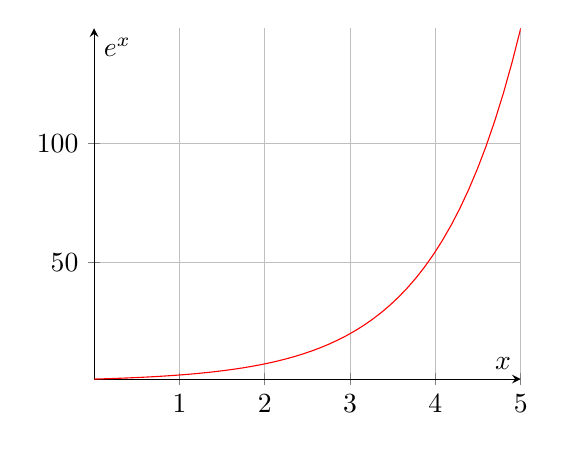
\begin{tikzpicture}
			\begin{axis}[domain=0:5, axis lines=middle, grid=both, xlabel=$x$, ylabel=$e^x$, width=7cm]
				\addplot[color=red, samples=50]{e^x};
			\end{axis}
		\end{tikzpicture}  
		\caption{Fonction exponentielle}
	\end{subfigure}
	\begin{subfigure}{0.45\textwidth}
		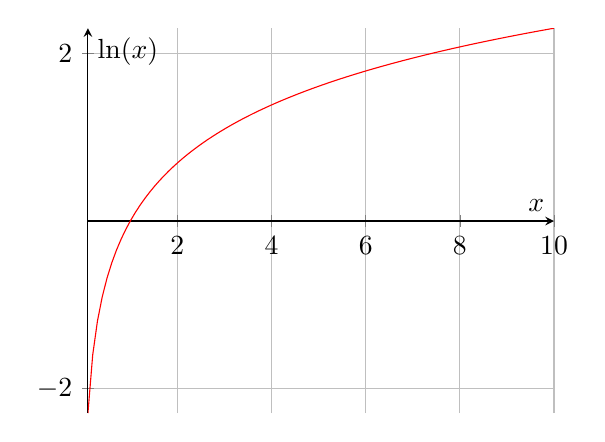
\begin{tikzpicture}
			\begin{axis}[domain=0:10, axis lines=middle, grid=both, xlabel=$x$, ylabel=$\ln(x)$, width=7.5cm]
				\addplot[color=red, samples=100]{ln(x)};
			\end{axis}
		\end{tikzpicture}
		\caption{Fonction logarithme népérien}
	\end{subfigure}
\end{figure}

\section{Fonctions hyperboliques}
\begin{graybox}
	\begin{definition}[Fonctions hyperboliques]
		On définit $\forall x \in \R$ 
		\begin{align*}
			\cosh(x) &= \frac{e^x + e^{-x}}{2} & \sinh(x) &= \frac{e^x - e^{-x}}{2} & \tanh(x) &= \frac{\sinh(x)}{\cosh(x)} = \frac{e^x - e^{-x}}{e^x + e^{-x}}
		\end{align*}
	\end{definition}
\end{graybox}

\begin{remarque}
	$\cosh = \mathrm{ch},\ \sinh = \mathrm{sh},\ \tanh = \mathrm{th}$
\end{remarque}

\begin{figure}[htbp]
	\centering
	\begin{subfigure}{0.3\textwidth}
		%\includegraphics[width=\textwidth, height=3.5cm]{images/ch.png}
		
		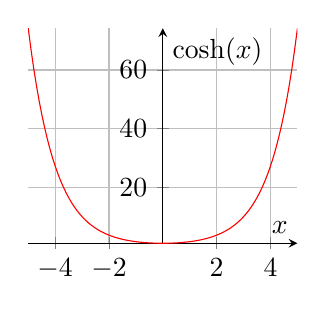
\begin{tikzpicture}
			\begin{axis}[domain=-5:5, axis lines=middle, grid=both, xlabel=$x$, ylabel=$\cosh(x)$, width=5cm]
				\addplot[color=red, samples=100]  {cosh(x)};
			\end{axis}
		\end{tikzpicture}
		\caption{Fonction cosh \cite{graphes}}
	\end{subfigure}
	\begin{subfigure}{0.3\textwidth}
		%\includegraphics[width=\textwidth, height=3.5cm]{images/sh.png}
		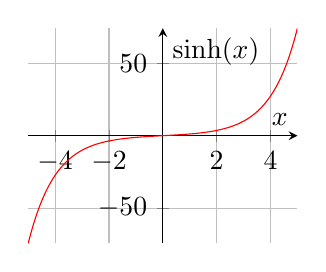
\begin{tikzpicture}
			\begin{axis}[domain=-5:5, axis lines=middle, grid=both, xlabel=$x$, ylabel=$\sinh(x)$, width=5cm]
				\addplot[color=red, samples=100]  {sinh(x)};
			\end{axis}
		\end{tikzpicture}
		\caption{Fonction sinh \cite{graphes}}
	\end{subfigure}
	\begin{subfigure}{0.3\textwidth}
		%\includegraphics[width=\textwidth, height=3.5cm]{images/tanh.png}
		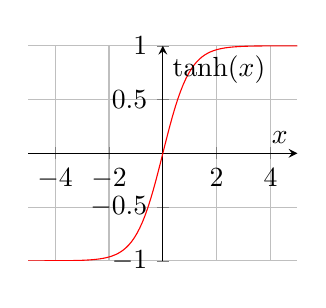
\begin{tikzpicture}
			\begin{axis}[domain=-5:5, axis lines=middle, grid=both, xlabel=$x$, ylabel=$\tanh(x)$, width=5cm]
				\addplot[color=red, samples=100]  {tanh(x)};
			\end{axis}
		\end{tikzpicture}
		\caption{Fonction tanh \cite{graphes}}
	\end{subfigure}
\end{figure}

\begin{table}[h!]
	\centering
	\begin{tabular}{c c c c}
		Fonction & ch & sh & th \\
		\hline
		Domaine de définition & $\R$ & $\R$ & $\R$ \\
		Parité & paire & impaire & impaire \\
		Dérivée & sh & ch & $1 - \mathrm{th}^2$ \\
		$\lim_{+\infty}$ & $+\infty$ & $+\infty$ & 1 \\
		$\lim_{-\infty}$ & $+\infty$ & $-\infty$ & -1 \\
		\hline
	\end{tabular}
\end{table}

\begin{graybox}
	\begin{proposition}[]
		$\forall x \in \R$
		\begin{align*}
			\cosh^2(x) - \sinh^2(x) = 1
		\end{align*}
	\end{proposition}
\end{graybox}

\begin{proof}
	\begin{align*}
		\cosh^2(x) - \sinh^2(x) &= \left( \frac{e^x + e^{-x}}{2} \right)^2 - \left( \frac{ e^x - e^{-x} }{ 2 } \right)^2 \\
		&= \frac{e^{2x} + 2 + e^{-2x} - (e^{2x} - 2 + e^{-2x})}{4} \\
		&= \frac{4}{4} \\
		&= 1
	\end{align*}
\end{proof}

\begin{graybox}
	\begin{proposition}[]
		$\forall x \in \R$
		\begin{align*}
			\tanh'(x) = 1 - \tanh^2(x)
		\end{align*}
	\end{proposition}
\end{graybox}

\begin{proof}
	$\tanh = \frac{\sinh}{\cosh}$
	\begin{align*}
		\tanh'(x) &= \frac{\sinh'(x)\cosh(x) - \sinh(x)\cosh'(x)}{\cosh^2(x)} \\
		&= \frac{\cosh^2(x) - \sinh^2(x)}{\cosh^2(x)} \\
		&= \frac{1}{\cosh^2(x)} = 1 - \tanh^2(x)
	\end{align*}
\end{proof}

\begin{graybox}
	\begin{proposition}[]
		$\forall x \in \R$ 
		\begin{align*}
			&\cosh{(x)} + \sinh{(x)} = \exp{(x)} \\
			&\cosh{(x)} - \sinh{(x)} = \exp{(-x)}
		\end{align*}
		On dit que $\cosh$ est la partie paire et $\sinh$ la partie impaire de l'exponentielle.
	\end{proposition}
\end{graybox}

\begin{graybox}
	\begin{proposition}[]
		$\forall (x, y) \in \R^2$
		\begin{align*}
			&1.\cosh{(x + y)} = \cosh{(x)}\cosh{(y)} + \sinh{(x)}\sinh{(y)} \\
			&2.\sinh{(x + y)} = \cosh{(x)}\sinh{(y)} + \sinh{(x)}\cosh{(y)}
		\end{align*}
	\end{proposition}
\end{graybox}

\begin{proof}
	1. 
	\begin{align*}
		\cosh{(x)}\cosh{(y)} + \sinh{(x)}\sinh{(y)} &= \left( \frac{e^x + e^{-x}}{2} \right) \left( \frac{e^y + e^{-y}}{2} \right) + \left( \frac{e^x - e^{-x}}{2} \right) \left( \frac{e^y - e^{-y}}{2} \right)\\
		&= \frac{e^x e^y + e^x e^{-y} + e^{-x}e^y + e^{-x} e^{-y}}{4} + \\ &\quad \frac{e^x e^y - e^x e^{-y} - e^{-x}e^y + e^{-x}e^{-y}}{4} \\
		&= \frac{2e^{x+y} + 2e^{-x-y}}{4} \\
		&= \frac{e^{x+y} + e^{-x-y}}{2} \\
		&= \cosh{(x + y)}
	\end{align*}
\end{proof}

\begin{remarque}
	En prenant $y = x$ on obtient :
	\begin{align*}
		\cosh{(2x)} &= \cosh^2{(x)} + \sinh^2{(x)} \\
		&= 1 + 2 \sinh^2{(x)} \\
		&= 2\cosh^2{(x)} - 1 \\
		\sinh{(2x)} &= 2\cosh{(x)} \sinh{(x)}
	\end{align*}
\end{remarque}


\begin{remarque}
	On verra avec les complexes :
	\begin{align*}
		\cos{x} &= \frac{e^{ix} + e^{-ix}}{2} & \sin{x} &= \frac{e^{ix} - e^{-ix}}{2}
	\end{align*}
	qui expliquent la parenté entre $\cos / \cosh$ et $\sin / \sinh$
\end{remarque}

\section{Fonctions puissance}
\par Dans quel cas peut-on définir $x^a$ ?

\begin{enumerate}
	\item Si $a \in \N, \forall x \in \R$
	\begin{align*}
		x^a = \underbrace{x \times x \times \cdots x}_{a \ fois}
	\end{align*}
	Par convention $x^0 = 1$
	\begin{align*}
		\begin{cases}
			\mathbb{R} &\to \mathbb{R} \\
			x &\mapsto x^a 
		\end{cases}
	\end{align*}
	est la fonction polynomiale de même parité que $a$.
	\item Si $a \in \mathbb{Z} \backslash \mathbb{N}$ et $x \neq 0$
	On pose 
	\begin{align*}
		x^a = \frac{1}{x^{-a}}
	\end{align*}
	\item Si $a = \frac{1}{n}$ pour $n \in \mathbb{N}^*$
	\begin{itemize}
		\item est la racine n-ième de $x$
		\item  $x^a$ est toujours défini quand $x \geqslant 0$, comme l'unique $y \in \mathbb{R}^+$ tel que $y^n = x$
		\item Si $n$ est impair : $x^a$ est défini pareillement pour tout $x \in \mathbb{R}$
	\end{itemize}
	\item Si $a \in \mathbb{R}$ et $x \in ]0, +\infty[$
	On pose : $x^a = \exp{(a \ln{x})}$ \\
	Les propriétés suivantes sont vraies dans tous les cas : 
	\begin{itemize}
		\item $1^a = 1$
		\item $x^a \cdot x^b = x^{a+b}$
		\item $(xy)^a = x^a y^a$
		\item $(x^a)^b = x^{ab}$
	\end{itemize}
	Si $x = e$, on retrouve la formule : $\exp{(a)}^b = \exp{(ab)}$
\end{enumerate}

\begin{graybox}
	\begin{proposition}[Dérivée de la fonction puissance]
		Soit la fonction :
		\begin{align*}
			f :
			\begin{cases}
				\mathbb{R}^*_+ &\to \mathbb{R} \\
				x &\mapsto x^a
			\end{cases}
		\end{align*}
		$f$ est dérivable et :
		\begin{align*}
			f'(x) &= \frac{a}{x} \exp{(a\ln{a})}  \\
			&= a x^{-1}x^a  \\
			&= a x^{a - 1}
		\end{align*}    
	\end{proposition}
\end{graybox}

\begin{exemple}
	Quelle est la dérivée de $g : x \mapsto 2^x$ ? \\
	On a : $g(x) = \exp{(x \ln{(2)})}$
	\begin{align*}
		g'(x) &= \ln{(2)} \exp{(x\ln{(2)})} \\
		g'(x) &= \ln{2} \cdot 2^x
	\end{align*}
\end{exemple}

\begin{graybox}
	\begin{theoreme}[Croissances comparées]
		$\forall n \in \N$
		\[\lim_{x \to +\infty} \frac{\exp{(ax)}}{x^b} = + \infty \]
		\[\lim_{x \to +\infty} \frac{x^b}{(\ln{x})^c} = +\infty\] 
		\[\lim_{x \to +\infty} \frac{\exp{(ax)}}{(\ln{x})^c} = +\infty\]
	\end{theoreme}
\end{graybox}
